\chapter*{Exponenciales y Logarítmicas}
\setcounter{chapter}{1}
\setcounter{section}{0}

\section{Función exponencial}
\blueBox{Definición}{
    Se llama \emph{función exponencial} a toda función $f : \R \rightarrow \R$ tal que 
    $$f(x) = a^x \text{ donde } a > 0 \text{ y } a \neq 1$$
}

Hay dos clases de funciones exponenciales:
\begin{enumerate}
    \item Cuando $a > 1$. Se llaman \emph{funciones exponenciales crecientes}.
    \item Cuando $0 < a < 1$. Se llaman \emph{funciones exponenciales decrecientes}.
\end{enumerate}

Cositas importantes: 
\begin{enumerate}
    \item Sus gráficas están por encima del eje $x \rightarrow Im(f) = \R^+$
    \item Cortan al eje $y$ en el punto $(0, 1)$ ya que $a^0 = 1$ sea cualquiera $a$
    \item Cuando $a > 1$ la función es estrictamente \textbf{creciente} y cuando $0 < a < 1$ es estrictamente \textbf{decreciente}
    \item No repiten puntos de la imagen
    \item {Hay una fórmula para calcular el valor de $f(x)$:
        $$f(x) = m \cdot a^x$$
        donde $m$ es el valor de $f(0)$
    }
\end{enumerate}

\section{Inversa de una función}
\blueBox{Definición}{
    Dada una función $f : A \rightarrow B$ se dice que su \emph{inversa} es una función $g : B \rightarrow A$ tal que:
    $$\text{si } f(a) = b \text{ entonces } g(b) = a \text{ (para toda $a \in A$)}$$
    Para denotar que $g$ es la inversa de $f$ se escribe 
    $$g = f^{-1}$$
}

\blueBox{Definición (inyectividad)}{
    Decimos que la función $f : A \rightarrow B$ es \emph{inyectiva} si 
    $$f(x_1) \neq f(x_2) \text{ siempre que } x_1 \neq x_2$$
    y para todo el dominio de $f$.
}
\blueBox{Definición (sobreyectividad)}{
    Decimos que la función $f : A \rightarrow B$ es \emph{sobreyectiva} si su codominio es igual a su imagen.
    $$B = Im(f)$$
}

\blueBox{Definición (biyectividad)}{
    Decimos que la función $f : A \rightarrow B$ es \emph{biyectiva} si es inyectiva y sobreyectiva.
}
Para que una función sea inversible tiene que ser biyecitva. Esto nos garantiza que al aplicar la inversa no haya más de una imagen por punto del dominio

\blueBox{Teorema}{
    Una función $f$ es inversible si y solo si es biyectiva. \textbf{TODAS LAS FUNCIONES EXPONENCIALES SON BIYECTIVAS}
}

\blueBox{Propiedad}{
    Si $f : A \subseteq \R \rightarrow B \subseteq \R$ es una función inversible, entonces las gráficas de $f$ y $f^{-1}$ son simétricas respecto al eje $y = x$.
}

\section{Funciones logarítmicas}
Considerando la función $f : \R \rightarrow \R^+ / f(x) = a^x \text{ con } a > 1$. \\
Esta función es inyectiva y sobreyectiva, por ende admite una inversa.

\blueBox{Definición (función logarítmica)}{
    Sea $f : \R \rightarrow \R^+ / f(x) = a^x \text{ con } a > 0 \text{ y } a \neq 1$ a la función $g: \R \rightarrow \R^+$ tal que $g = f^{-1}$, se la denomina \emph{función logarítmica en base a}.
    $$g : \R \rightarrow \R^+ / g(x) = log_a(x)$$
    $$log_a(x) = y \Leftrightarrow a^y = x$$
}
\subsection{Propiedades}
En todos estos casos se supone que $a > 0$, $a \neq 1$ y $x, y > 0$.
\begin{enumerate}
    \item $log_a 1 = 0$ ya que $a^0 = 1$
    \item $log_a a = 1$ ya que $a^1 = a$
    \item $log_a(x \cdot y) = log_a x + log_a y$
    \item $log_a \left(\frac{x}{y}\right) = log_a x - log_a y$
    \item $log_a x^n = n \cdot log_a x$
    \item $a^{log_a x} = x$
\end{enumerate}


\subsection{log y ln}
Las notaciones son las siguientes:
\begin{center}
    $log$ para denotar al $log_{10}$ (logaritmo en base 10)\\
    $ln$ para denotar al $log_e$ (logaritmo natural)
\end{center}

\subsection{Cambio de base}
Se puede cambiar la base de un logatirmo de la siguiente manera:
$$\boxed{log_b x = \frac{log_a x}{log_a b}}$$

\textbf{Ejemplo}: 
$$log_4 32 = \frac{log_2 32}{log_2 4} = \frac{log_2 2^5}{log_2 2^2} = \frac{5 log_2 2}{2 log_2} = \frac{5}{2} = 2,5$$
Usando la calculadora:
$$log_4 32 = \frac{ln 32}{ln 4} = 2,5$$

\section{¿Como encontrar la inversa de una función?}
Ejemplo:

$$P = 100 \cdot 2^t$$
Hay que "despejar" $t$ para poder encontrar la inversa de la función.
$$P = 100 \cdot 2^t \Leftrightarrow \frac{P}{100} = 2^t \Leftrightarrow \ln \left(\frac{P}{100}\right) = \ln 2^t \Leftrightarrow \ln \left(\frac{P}{100}\right) = t \ln 2$$
$$t = \frac{\ln \left(\frac{P}{100}\right)}{\ln 2}$$

\section{Las funciones $f(x) = e^x$ y $g(x) = \ln x$}

% graph with e^x and ln x with tikzpicture and axis
\begin{center}
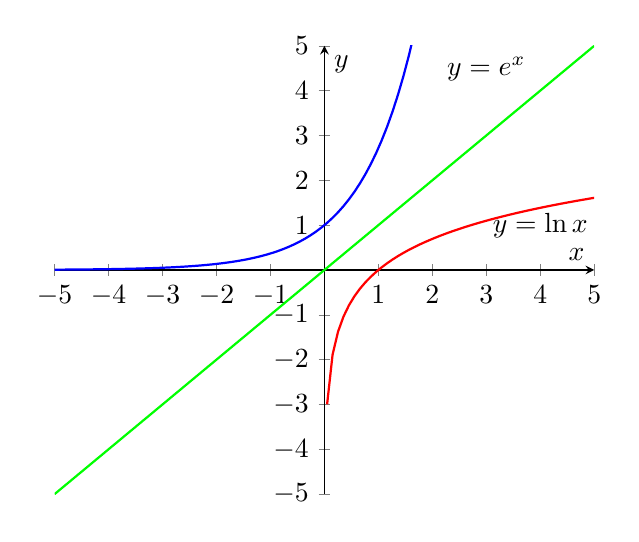
\begin{tikzpicture}
    \begin{axis}[
        xmin=-5, xmax=5,
        ymin=-5, ymax=5,
        axis lines=middle,
        xtick={-10,-9,-8,-7,-6,-5, -4, -3, -2, -1, 0, 1, 2, 3, 4, 5, 6, 7, 8, 9, 10},
        ytick={-10,-9,-8,-7,-6,-5, -4, -3, -2, -1, 0, 1, 2, 3, 4, 5, 6, 7, 8, 9, 10},
        xlabel=$x$,
        ylabel=$y$,
        legend pos=north west,
        legend cell align=left,
        ]
        \addplot[domain=-5:5, samples=100, color=blue, thick] {exp(x)};
        \addplot[domain=-5:5, samples=100, color=red, thick] {ln(x)};
        \addplot[domain=-5:5, samples=100, color=green, thick] {x};
        % nodes for the functions
        \node[above] at (axis cs:3, 4) {$y = e^x$};
        \node[above] at (axis cs:4, 0.5) {$y = \ln x$};

    \end{axis}
\end{tikzpicture}
\end{center}

Son simétricos respecto al eje $y = x$.\\

Propiedades de los \textbf{logaritmos naturales con base > 1}:
\begin{enumerate}
    \item El dominio de $g$ es $\R^+$
    \item Su conjunto imagen es $\R$
    \item Es estrictamente creciente
    \item La recta $x = 0$ es asíntota vertical de $g$
    \item $g(x) = \ln x$ corta al eje de abscisas en $x = 1$ 
\end{enumerate}

\section{Ecuaciones exponenciales y logarítmicas}

Ejemplo: 
$$3^{2x-1} = \frac{1}{9}$$
Para resolverla hay distintas estrategias:
\begin{enumerate}
    \item {Usar propiedades de potencias para tener todo en una misma base
    $$3^{2x-1} = \frac{1}{9} \Leftrightarrow 3^{2x-1} = 3^{-2}$$
    Como las bases son iguales, se igualan los exponentes:
    $$2x-1 = -2$$
    por ende $x = -\frac{1}{2}$
    }
    \item {Usar logaritmos:
        $$3^{2x-1} = \frac{1}{9} \Leftrightarrow log_3 3^{2x-1} = log_3 \frac{1}{9} \Leftrightarrow (2x-1) log_3 3 = log_3 1 - log_3 9$$
        $$\Leftrightarrow (2x-1) = 0 - 2 \Leftrightarrow x = -\frac{1}{2}$$
    }
\end{enumerate}